
\chapter{Light collection efficiency of an objective}
\markboth{\MakeUppercase{Appendix C}}{}

\setcounter{table}{0}
\renewcommand{\thetable}{C\arabic{table}}

\label{app:lightEff}
\graphicspath{{./figures/2_DualMouse/}}

    Let's define light collection efficiency $\eta$ as the ratio of collected photons and all emitted photons:
    \[
    \eta = \frac{N_{collected}}{N_{emitted}}
    \]
    Since we can assume that the direction of photons emitted from a fluorescent molecule are random, the light collection efficiency will correspond to the solid angle subtended by the objective front lens at the focal point. To calculate this, let's consider the unit sphere centered at the focal point, and calculate the surface area of the spherical cap corresponding to the objective acceptance angle $\alpha$ (Fig. \ref{fig:light_effa}). The area of the cap can be expressed as a function of the angle:
    \[
    A_{cap} = 2\pi r^2 (1-\cos \alpha)
    \]
    The surface area of the full sphere is calculated as:
    \[
    A_{sph} = 4 \pi r^2
    \]
    For both equations $r$ is the radius of the sphere. From here, the light collection efficiency can be calculated as:
    \[
    \eta = \frac{N_{collected}}{N_{emitted}} = \frac{A_{cap}}{A_{sph}} = \frac{1-\cos \alpha}{2}
    \]
    As most objectives are characterized by the numerical aperture, we also plot $\eta$ as a function of the NA on \autoref{fig:light_effb}.

    \begin{figure}[tpb]
      \centering
    \begin{subfigure}[t]{0.39\textwidth}
      \centering
      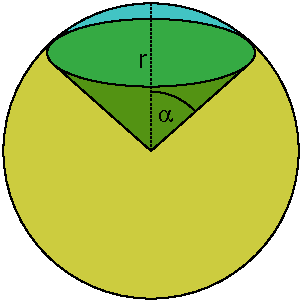
\includegraphics[page=1,width=0.8\textwidth]{efficiency/sphere}
      \caption{\textbf{}}
      \label{fig:light_effa}
    \end{subfigure}
    \begin{subfigure}[t]{0.39\textwidth}
      \centering
      \includegraphics[page=1,width=1\textwidth]{efficiency/light_eff}
      \caption{\textbf{}}
      \label{fig:light_effb}
    \end{subfigure} 
    \bcaption[Light collection efficiency of an objective]{\textbf{(a)} Light collection efficiency is the ratio of photons collected by the objective and all emitted photons. If the fluorophores are emitted randomly in all directions, it will be the surface ratio of the conical section (blue) to the whole sphere. \textbf{(b)} Light collection efficiency ($\eta$) as a function of the numerical aperture (NA).}
    \label{fig:light_eff}
    \end{figure}